\documentclass[12pt, varwidth]{standalone}
\usepackage{tikz}
\usepackage{pgfplots}
\usepackage{amsmath}
\usepackage{geometry}
\geometry{a4paper, margin=1in}

\pgfplotsset{compat=1.18}

\begin{document}

    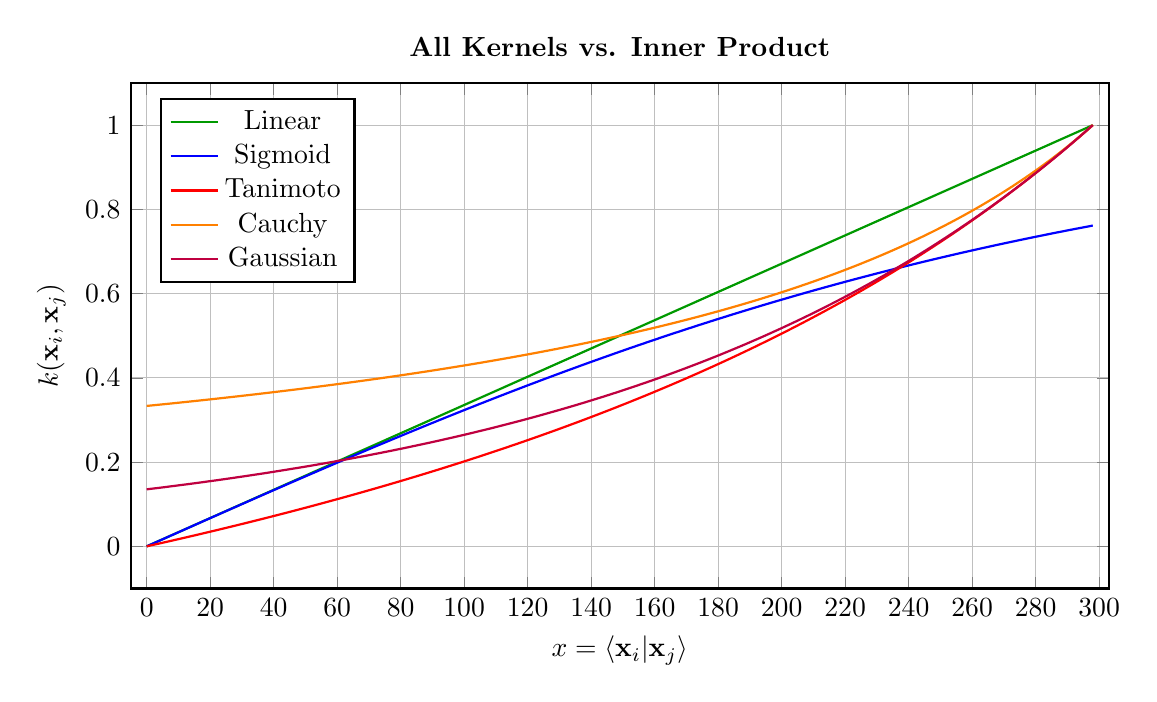
\begin{tikzpicture}
        \begin{axis}[
            title={\textbf{All Kernels vs. Inner Product}},
            xlabel={$x = \langle \textbf{x}_i | \textbf{x}_j \rangle$},
            ylabel={$k(\textbf{x}_i, \textbf{x}_j)$},
            domain=0:298,        % Bounded by the minimum and maximum possible matches
            samples=200,
            xmin=-5, xmax=303,
            ymin=-0.1, ymax=1.1,
            legend pos=north west,
            grid=both,
            minor grid style={lightgray},
            width=14cm, height=8cm,
            thick
        ]
        
        % Linear function
        \addplot [color=green!60!black] {x / 298};
        \addlegendentry{Linear}

        % Sigmoid function
        \addplot [color=blue] {tanh(x / 298)};
        \addlegendentry{Sigmoid}
        
        % Tanimoto function
        \addplot [color=red] {x / (596 - x)};
        \addlegendentry{Tanimoto}

        % Cauchy function translated (d^2 replaced with 596 - 2x)
        \addplot [color=orange] {298 / (298 + (596 - 2*x))};
        \addlegendentry{Cauchy}
        
        % Gaussian function translated (d^2 replaced with 596 - 2x)
        \addplot [color=purple] {exp(-(596 - 2*x) / 298)};
        \addlegendentry{Gaussian}

        \end{axis}
    \end{tikzpicture}

    \vspace{1cm}

    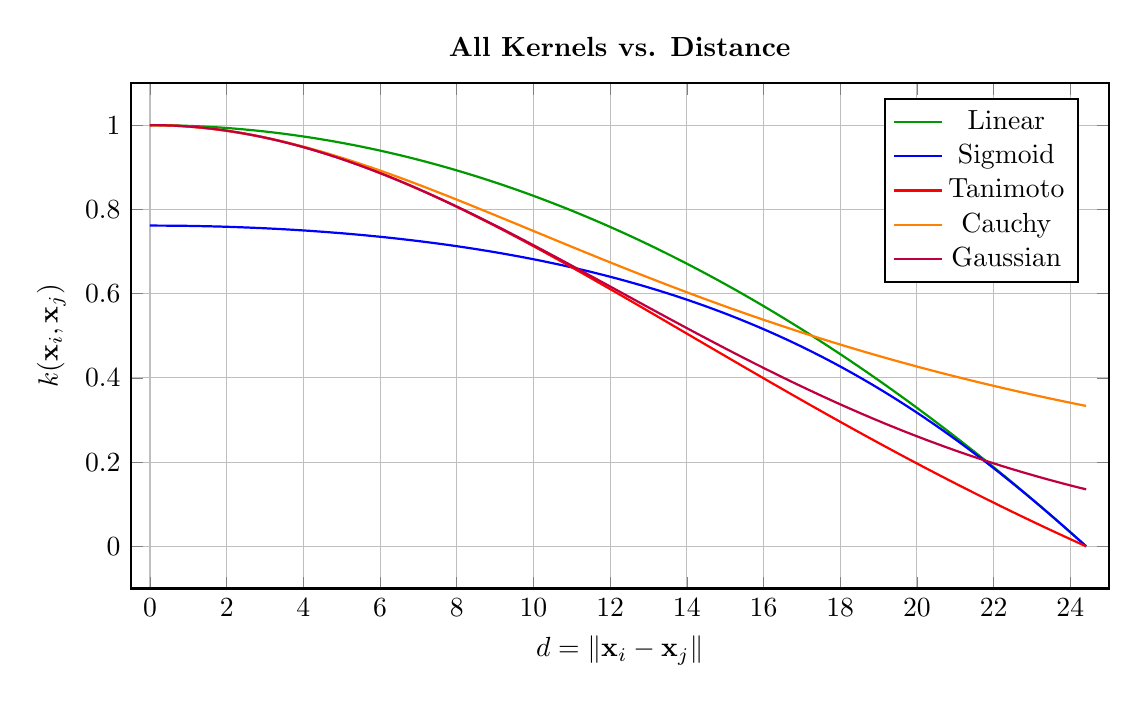
\begin{tikzpicture}
        \begin{axis}[
            title={\textbf{All Kernels vs. Distance}},
            xlabel={$d = \| \textbf{x}_i - \textbf{x}_j \|$},
            ylabel={$k(\textbf{x}_i, \textbf{x}_j)$},
            domain=0:24.413,      % Bounded by sqrt(596), the max possible distance
            samples=200,
            xmin=-.5, xmax=25,
            ymin=-0.1, ymax=1.1,
            legend pos=north east,
            grid=both,
            minor grid style={lightgray},
            width=14cm, height=8cm,
            thick
        ]
        
        % Linear function translated (x replaced with 298 - d^2/2)
        \addplot [color=green!60!black] {(298 - x^2/2) / 298};
        \addlegendentry{Linear}

        % Sigmoid function translated (x replaced with 298 - d^2/2)
        \addplot [color=blue] {tanh((298 - x^2/2) / 298)};
        \addlegendentry{Sigmoid}

        % Tanimoto function translated (x replaced with 298 - d^2/2)
        \addplot [color=red] {(298 - x^2/2) / (596 - (298 - x^2/2))};
        \addlegendentry{Tanimoto}

        % Cauchy function
        \addplot [color=orange] {298 / (298 + x^2)};
        \addlegendentry{Cauchy}
        
        % Gaussian function
        \addplot [color=purple] {exp(-x^2 / 298)};
        \addlegendentry{Gaussian}

        \end{axis}
    \end{tikzpicture}

\end{document}